\documentclass{beamer}
\usepackage{mathrsfs,xcolor,setspace,comment,centernot,listings,framed,subfig,ragged2e}
\usepackage[utf8]{inputenc}
\usepackage[T1]{fontenc}

\DeclareMathOperator{\Cov}{Cov}
\DeclareMathOperator{\Var}{Var}
\DeclareMathOperator{\E}{\mathbb{E}}
\DeclareMathOperator{\Proba}{\mathbb{P}}

\newcommand{\Covb}[2]{\ensuremath{\Cov\!\left[#1,#2\right]}}
\newcommand{\Eb}[1]{\ensuremath{\E\!\left[#1\right]}}
\newcommand{\Pb}[1]{\ensuremath{\Proba\!\left[#1\right]}}
\newcommand{\Varb}[1]{\ensuremath{\Var\!\left[#1\right]}}

% norm
\newcommand{\norm}[1]{\| #1 \|}

\newcommand{\indep}{\rotatebox[origin=c]{90}{$\models$}}



% config du theme metropolis
\usetheme[progressbar=frametitle,block=fill, titleformat=smallcaps,sectionpage=progressbar,]{metropolis}



\title{Mapping the integration between Knowledge Domains in Theoretical and Quantitative Geography}
\subtitle{}

\date{11/09/2025\\
\textbf{ECTQG 2025}\\
Special Session: Theoretical Geography\\
and the History of Geography}

\author{Juste Raimbault\textsuperscript{1,2,3,4}}
\institute{\textsuperscript{1}LaSTIG, IGN-ENSG-UGE\\
\textsuperscript{2}CASA, UCL\\
\textsuperscript{3}UPS CNRS 3611 ISC-PIF\\
\textsuperscript{4}UMR CNRS 8504 Géographie-cités
}



%definition de la couleur du texte dans la balise \alert{}
\definecolor{vertIGN}{HTML}{96C31E} % vert IGN %vrai valeur #97BE0D
\setbeamercolor{alerted text}{fg=vertIGN}

\definecolor{grisIGN}{HTML}{22292F} % Gris IGN tiré vers le noir 
\setbeamercolor{background canvas}{bg=grisIGN}


% code pour placer le log ENSG dans le bandeau de titre 
\makeatletter
\setbeamertemplate{frametitle}{%
  \nointerlineskip%
  \begin{beamercolorbox}[%
      wd=\paperwidth,%
      sep=0pt,%
      leftskip=\metropolis@frametitle@padding,%
      rightskip=\metropolis@frametitle@padding,%
    ]{frametitle}%
  \metropolis@frametitlestrut@start%
  \insertframetitle%
  \nolinebreak%
  \metropolis@frametitlestrut@end%
  \hfill
  \raisebox{-0.6ex}{
\includegraphics[height=4ex,keepaspectratio]{figures/logoENSG_small.jpg}}
  \end{beamercolorbox}%
}


\newcommand{\noun}[1]{\textsc{#1}}
\newcommand{\jitem}[1]{\item \begin{justify} #1 \end{justify} \vfill{}}
\newcommand{\sframe}[2]{\frame{\frametitle{#1} #2}}

\newenvironment{centercolumns}{\begin{columns}[c]}{\end{columns}}
%\newenvironment{jitem}{\begin{justify}\begin{itemize}}{\end{itemize}\end{justify}}



\usepackage{pifont}
\newcommand{\cmark}{\ding{51}}
\newcommand{\xmark}{\ding{55}}


\usepackage{multirow}

\makeatother




% logo ENSG première page 
\titlegraphic{\vspace{4cm}\flushright
\includegraphics[width=2cm,height=2cm]{figures/logoENSG_big.png}} 





\begin{document}
\metroset{background=dark} % change background theme according to manual
\maketitle	







\sframe{History of ECTQG}{

% Theoretical and Quantitative Geography (TQG), since its inception in Europe in the 70s as a scientific current [Cuyala, 2015], has always been motivated by a strong integration between quantitative studies (empirical or modeling) and theoretical constructions.

% -> illustration map Cuyala?

\begin{center}
	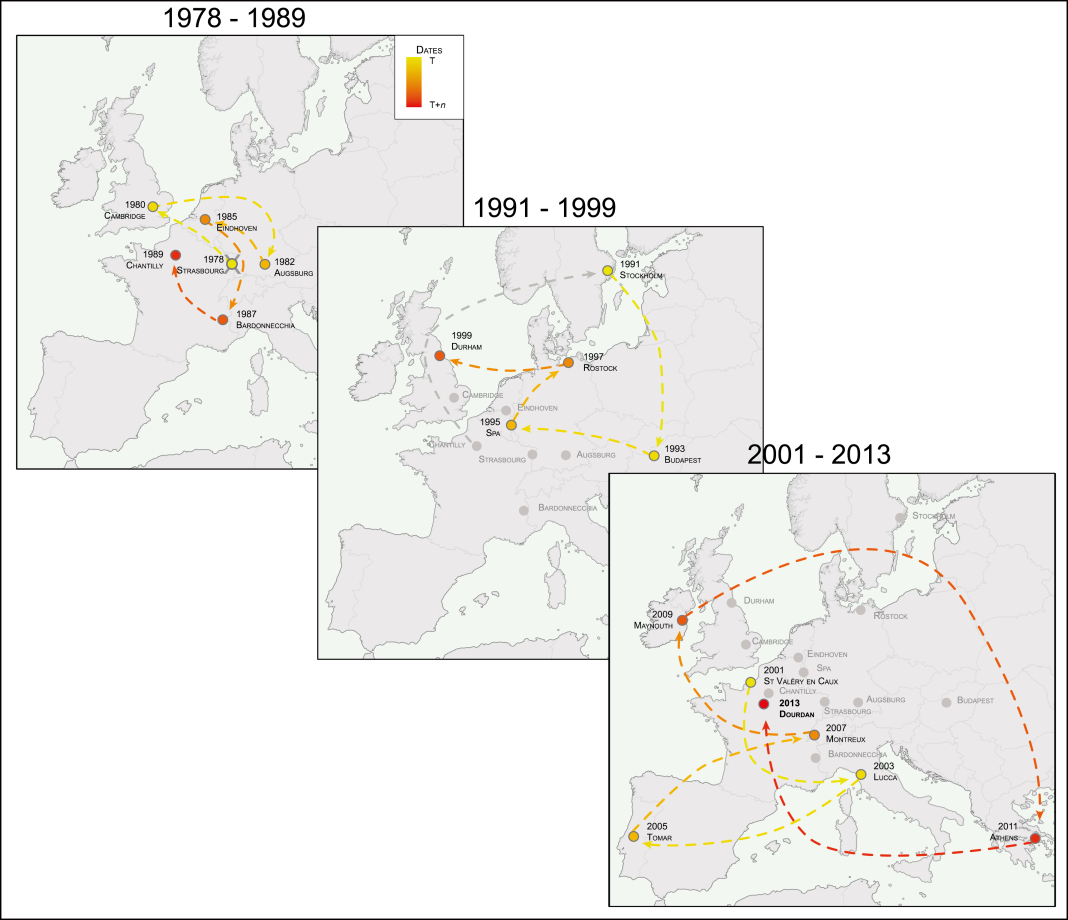
\includegraphics[height=0.8\textheight]{figures/Cuyala2016_img-2.png}
\end{center}

\footnotesize

\textit{Diversity and integration of Theoretical and Quantitative Geography \cite{cuyala2016spatial}.}


}

\sframe{Quantitative epistemology}{

% autre illustration et pub pour CybergeoNetworks (et projets en cours)


\begin{center}
	\includegraphics[height=0.6\textheight]{../../../../../Cybergeo/Docs/arxiv/v2/fig6.jpg}
\end{center}

\footnotesize

\textit{Spatialised bibliometrics as a tool for a more reflexive and open science: CybergeoNetworks project \cite{raimbault2021empowering}, continued into OpenJournalScope (currently submitted to FNSO).}

\url{https://analytics.huma-num.fr/geographie-cites/cybergeonetworks/}

}

\sframe{Knowledge domains}{

% [Livet et al., 2010] have conceptualised, for activities implying modelling in social science in general, a strong integration between three Knowledge Domains, namely Theory, Empirical, and Modelling. This Knowledge Framework has been refined by [Raimbault, 2017] with the addition of other domains with a key importance in TQG: Data, Methods, and Tools.


% slides before had white background -> convert
%convert -density 150 -resize 1000x -background white -flatten ../../../../../../NetworksTerritories/CityNetwork/Docs/Papers/KnowledgeFramework/arxiv/v1/framework.pdf figures/framework.png


\begin{center}
	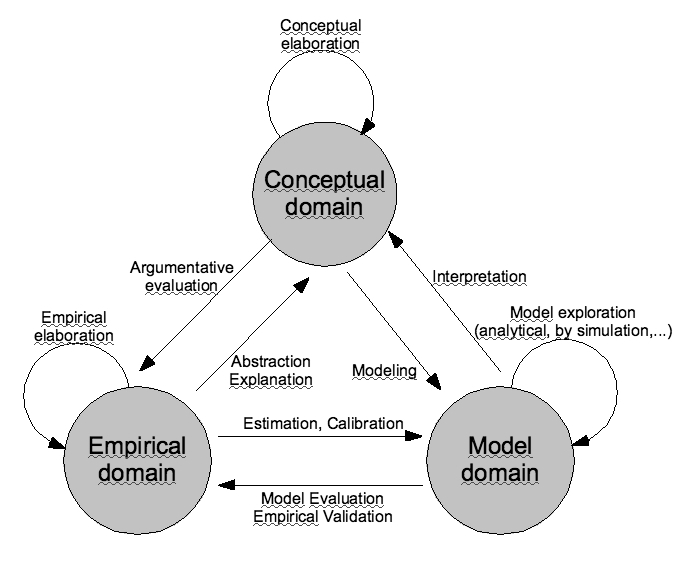
\includegraphics[height=0.55\textheight]{figures/Livet2010_Figure1.jpg}%\hspace{0.1cm}
	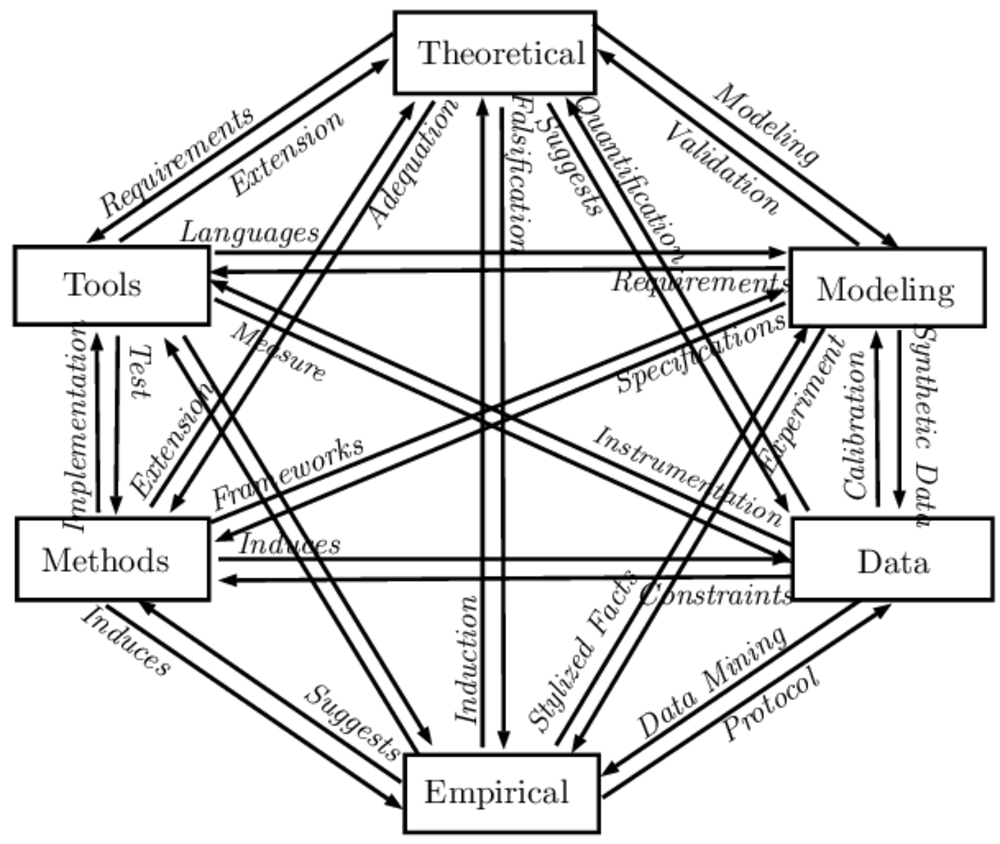
\includegraphics[height=0.55\textheight]{figures/framework.png}
\end{center}

\medskip

\textit{(Left) Knowledge framework for agent-based modelling by \cite{livet2010ontology}; (Right) Refinement with more Knowledge Domains (KDs) by \cite{raimbault2017applied}.}


}

\sframe{KDs in Pumain's Evolutionary Urban Theory}{

% transparent background -> convert
%convert -background white -flatten /home/JRaimbault/ComplexSystems/NetworksTerritories/CityNetwork/Docs/Communications/2017/CSDM2017/figures/openmoleslide.png figures/kd_evolth.png

% second slide with previous work on Denise's theory?

\begin{center}
	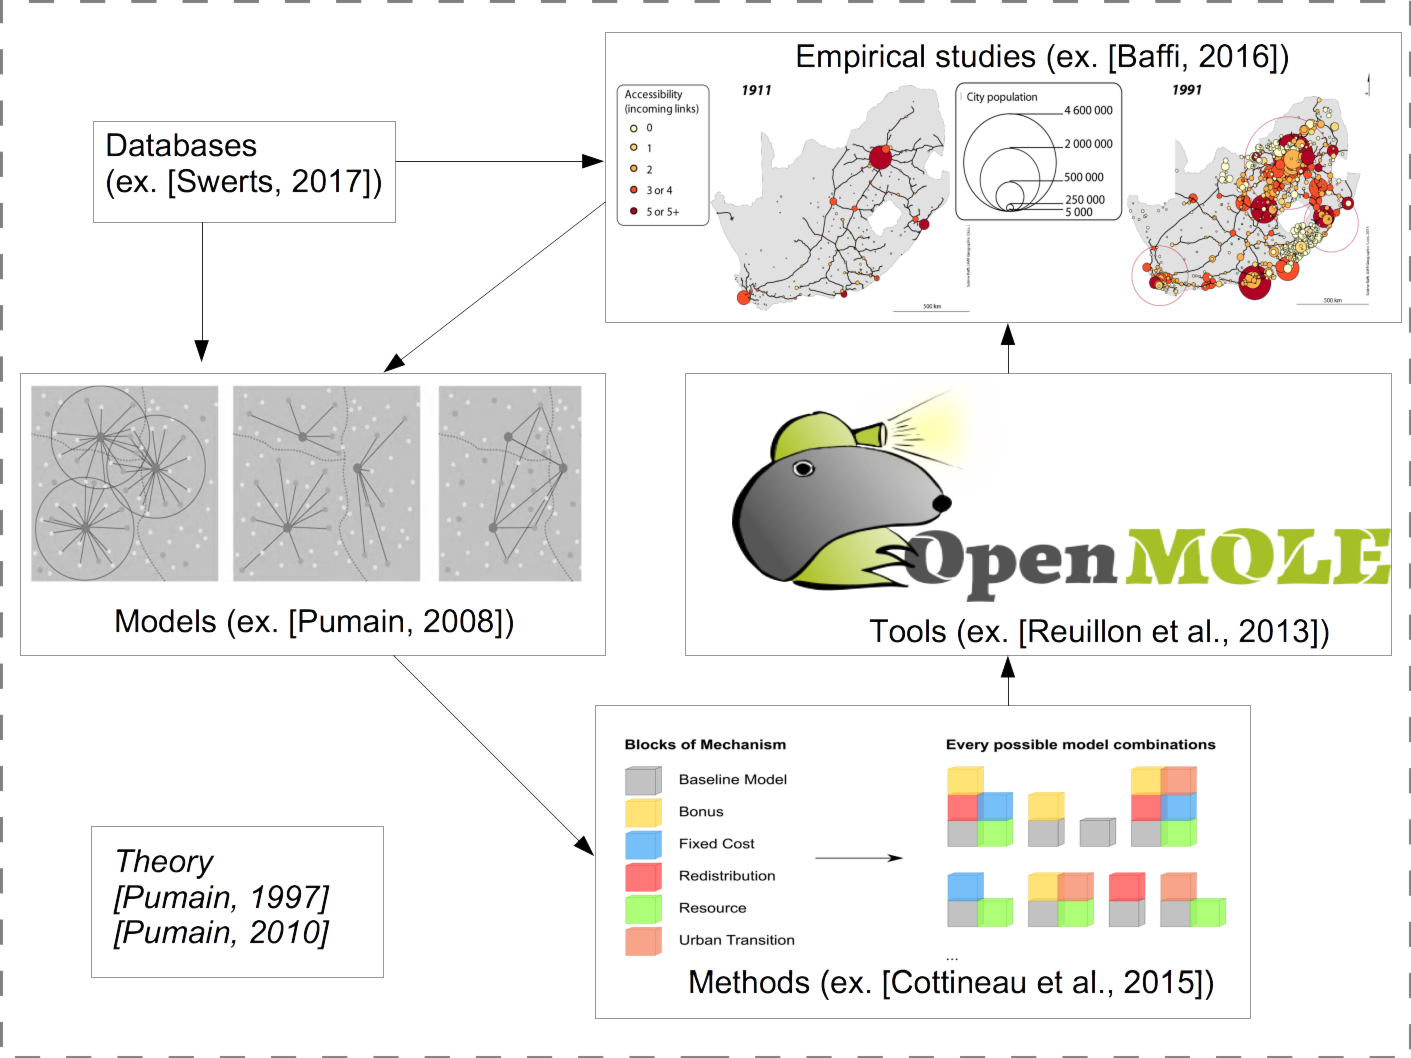
\includegraphics[height=0.8\textheight]{figures/kd_evolth.png}
\end{center}

\footnotesize

\cite{raimbault2017applied}

}


\sframe{Research objective}{


% To what extent theories in TQG (in the sense of bodies of knowledge) effectively involve a variety of Knowledge Domains, and mobilises them in an integrated way to produce knowledge?
% We propose in this contribution to investigate this question for two case studies:


% ! add a disclaimer on def of theory? - be careful when annotate the papers!



$\rightarrow$ previous work on Pumain's Evolutionary Urban Theory \cite{pumain2018evolutionary} by \cite{raimbault2017applied} suggested an integration of KDs

\medskip

$\rightarrow$ more general ongoing epistemological research on TQG: \cite{raimbault2017co} (TheoQuant 2017), \cite{raimbault2017invisible} (ECTQG 2017), \cite{raimbault2018extracting} (CCS 2018), \cite{raimbault:halshs-02284848} (ECTQG 2019), \cite{raimbault:halshs-02441891} (CCS 2019)

\bigskip

\textbf{Research objective:}

\textit{}


}


\sframe{Data: case studies}{

% Pumain’s evolutionary theory for systems of cities [Pumain, 2018] (which has been developed the last 30 years, is an example of a fruitful TQG approach, and is rather well delimited), and studies of Zipf’s law for the size of cities [Cottineau, 2017] (with a longer history, and a less delimited context with several disciplines involved from economics to regional science, physics and geography).



}

\sframe{Data collection: corpus construction}{

%Starting from an initial corpus for each case (foundational papers for the Evolutionary Theory, and around fifty papers found by [Cottineau, 2017] in a systematic review), we reconstruct backward citation networks up to depth two using the bibilographic tools provided by [Raimbault, 2019]. We use these citation networks as corpuses in which integration between knowledge domains is studied.

% EvUrbTh: 16333 nodes, 21775 edges ; core (deg > 2) : 1252 4950




}


\sframe{Data consolidation: manual annotation}{

%Given the relatively small size of corpuses (≃100 and 500 papers), it is much robust to tag papers for knowledge domains by hand.


% reflexion on using a ML approach - anyway would need training data (this could be a base corpus for a more systematic study) - pb: how to delineate TQG? using ECTQG proceedings!

% Counts for evurbth: / 1252
%      data empirical    method     model    theory      tool    NA
%        2       208       108       387       456        17     74





}


\sframe{Results: citation networks}{


\begin{center}
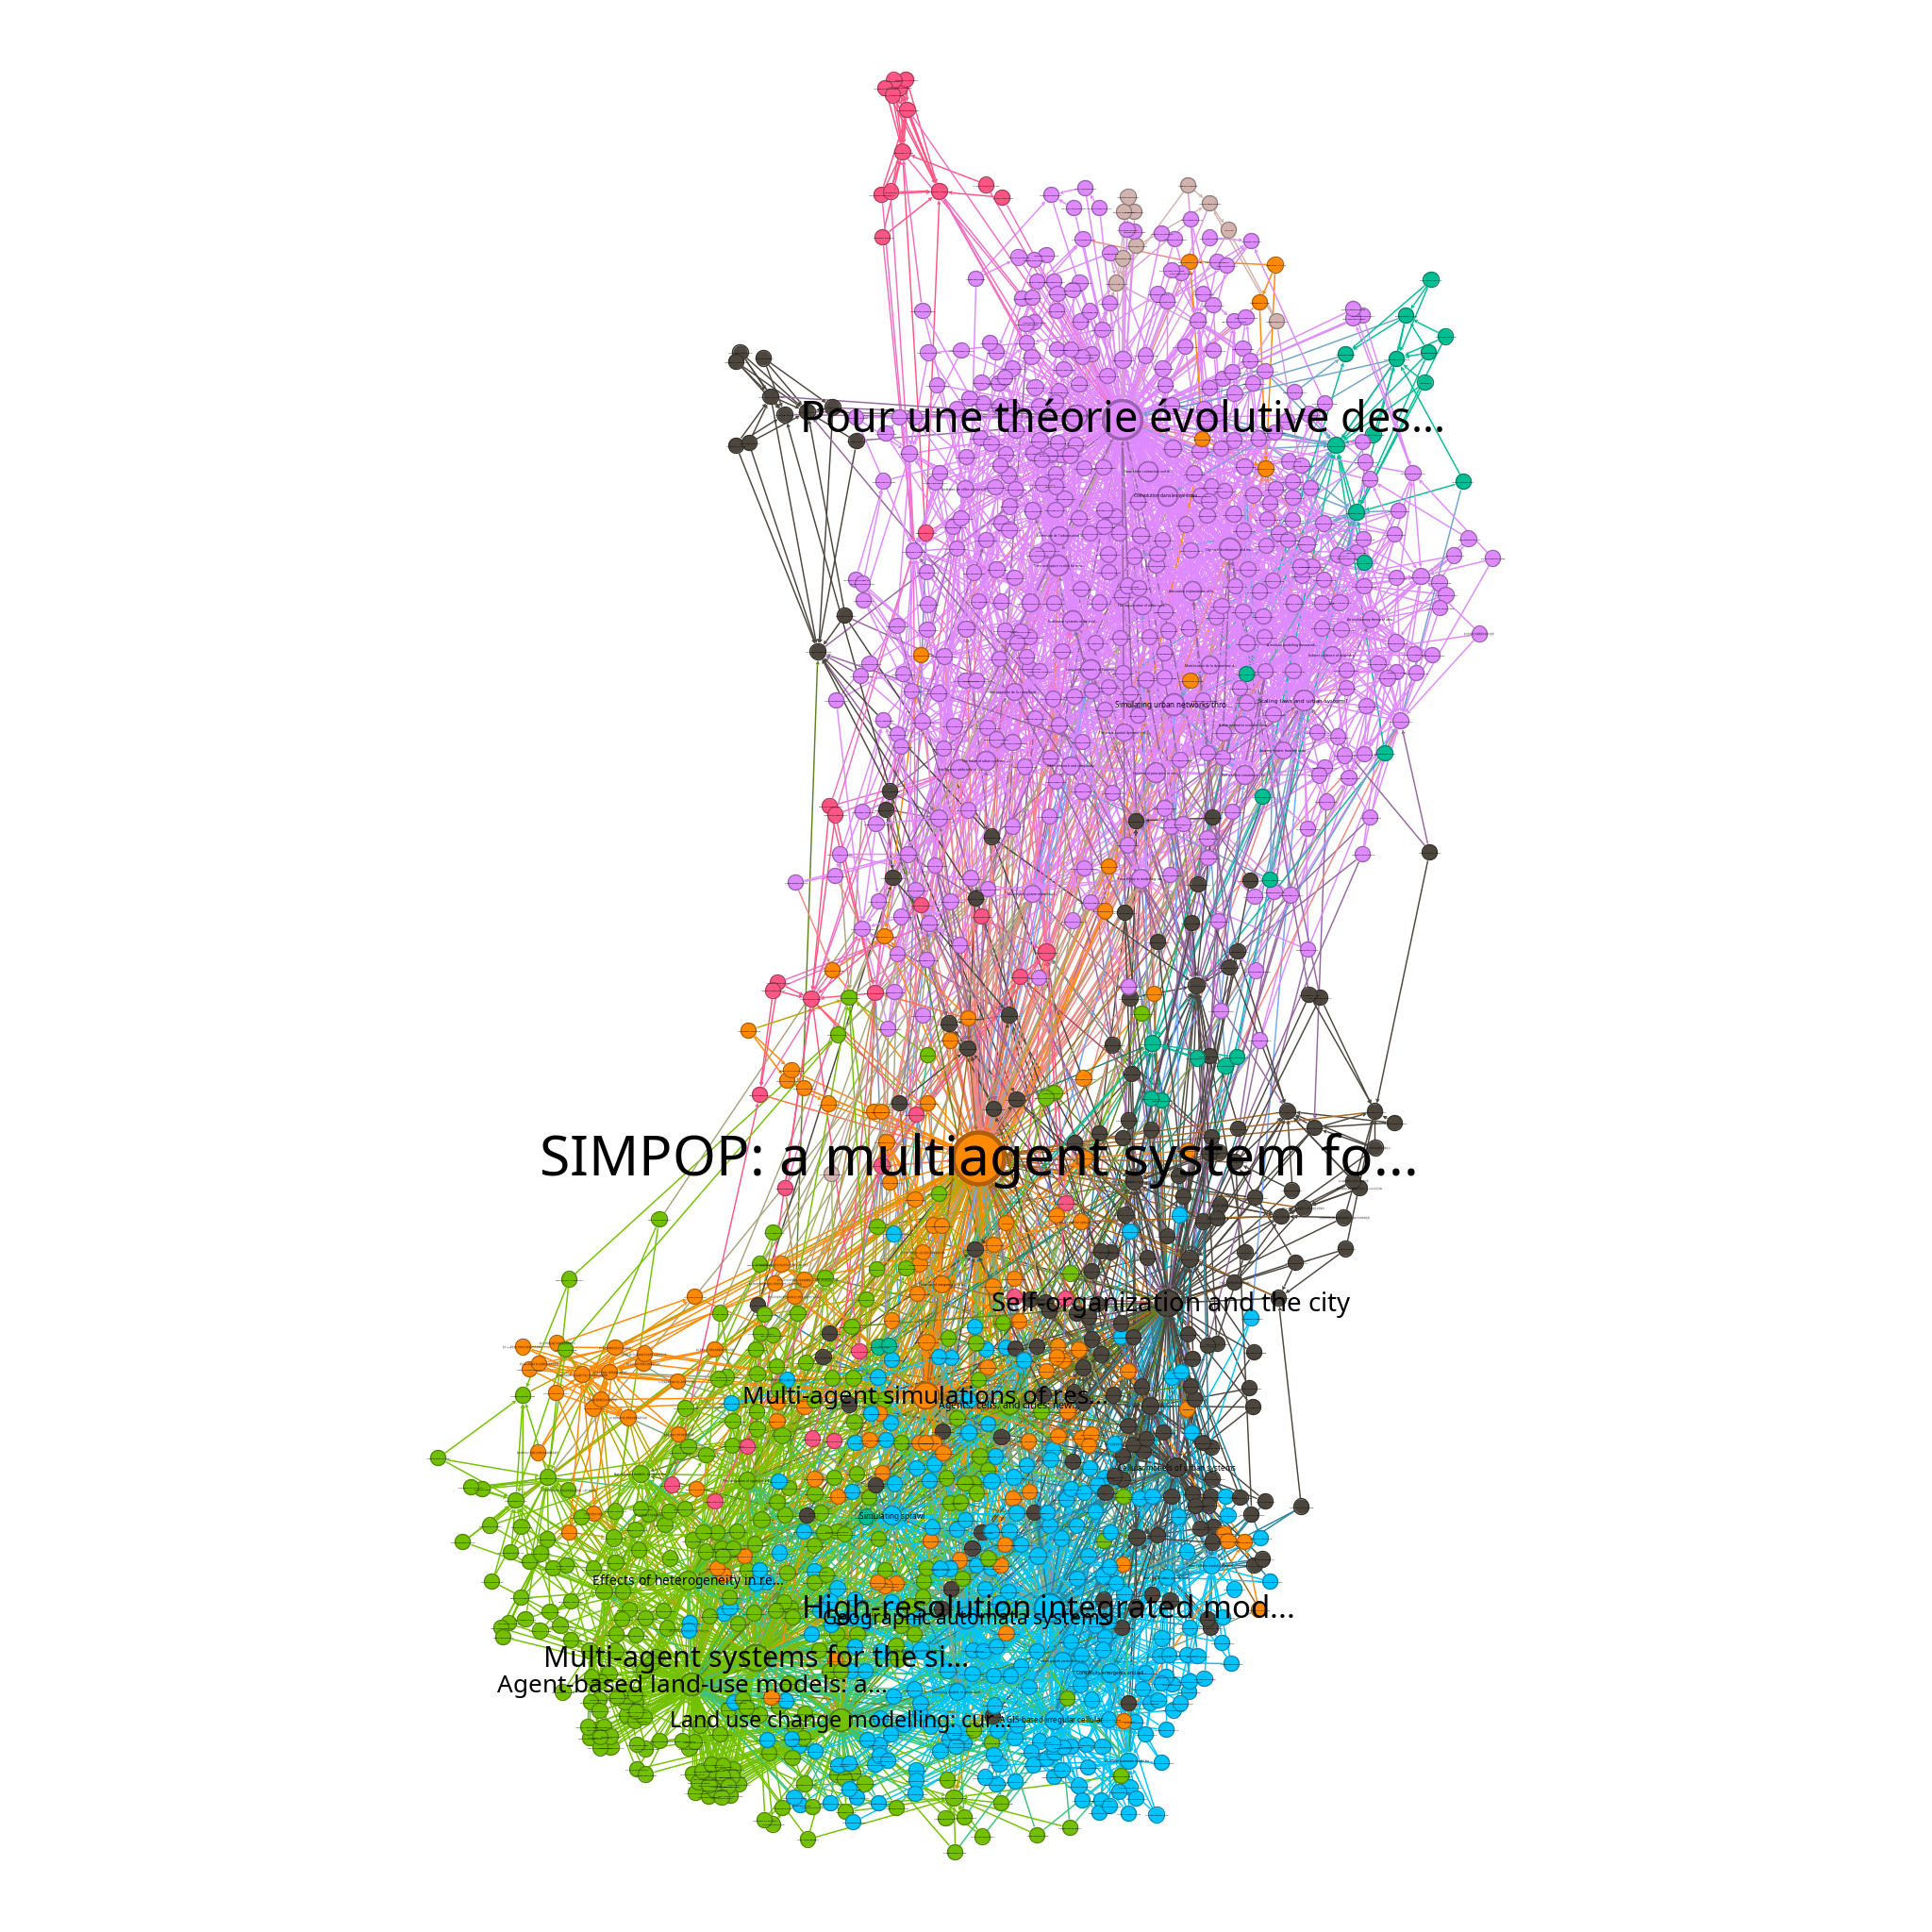
\includegraphics[width=0.48\linewidth]{../../../../Results/core_evurbth.png}
\end{center}


\footnotesize

\textit{(Left) Evolutionary Urban Theory; (Right) Zipf}


}

\sframe{Results:community detection}{

% intercommunity citations flows

\begin{center}
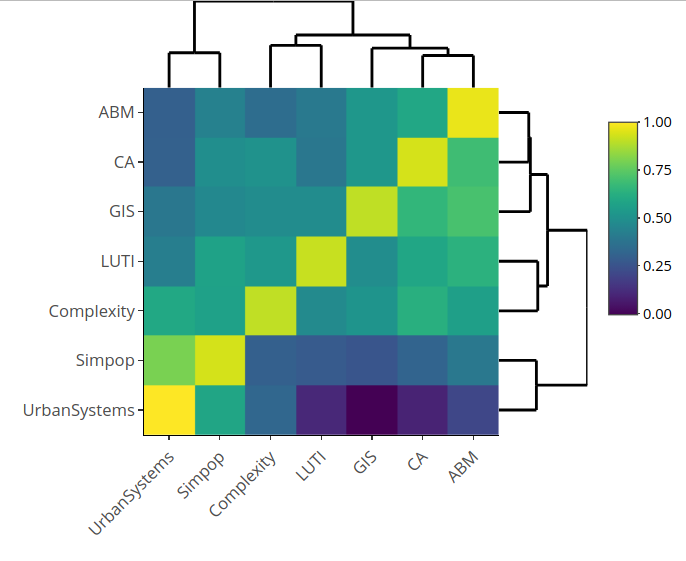
\includegraphics[width=0.48\linewidth]{../../../../Results/evurbth_communities-citations.png}
\end{center}


\footnotesize

\textit{(Left) Evolutionary Urban Theory; (Right) Zipf}

}


\sframe{Results: KDs composition}{

% bar stack of KDs proportions in each community

\begin{center}
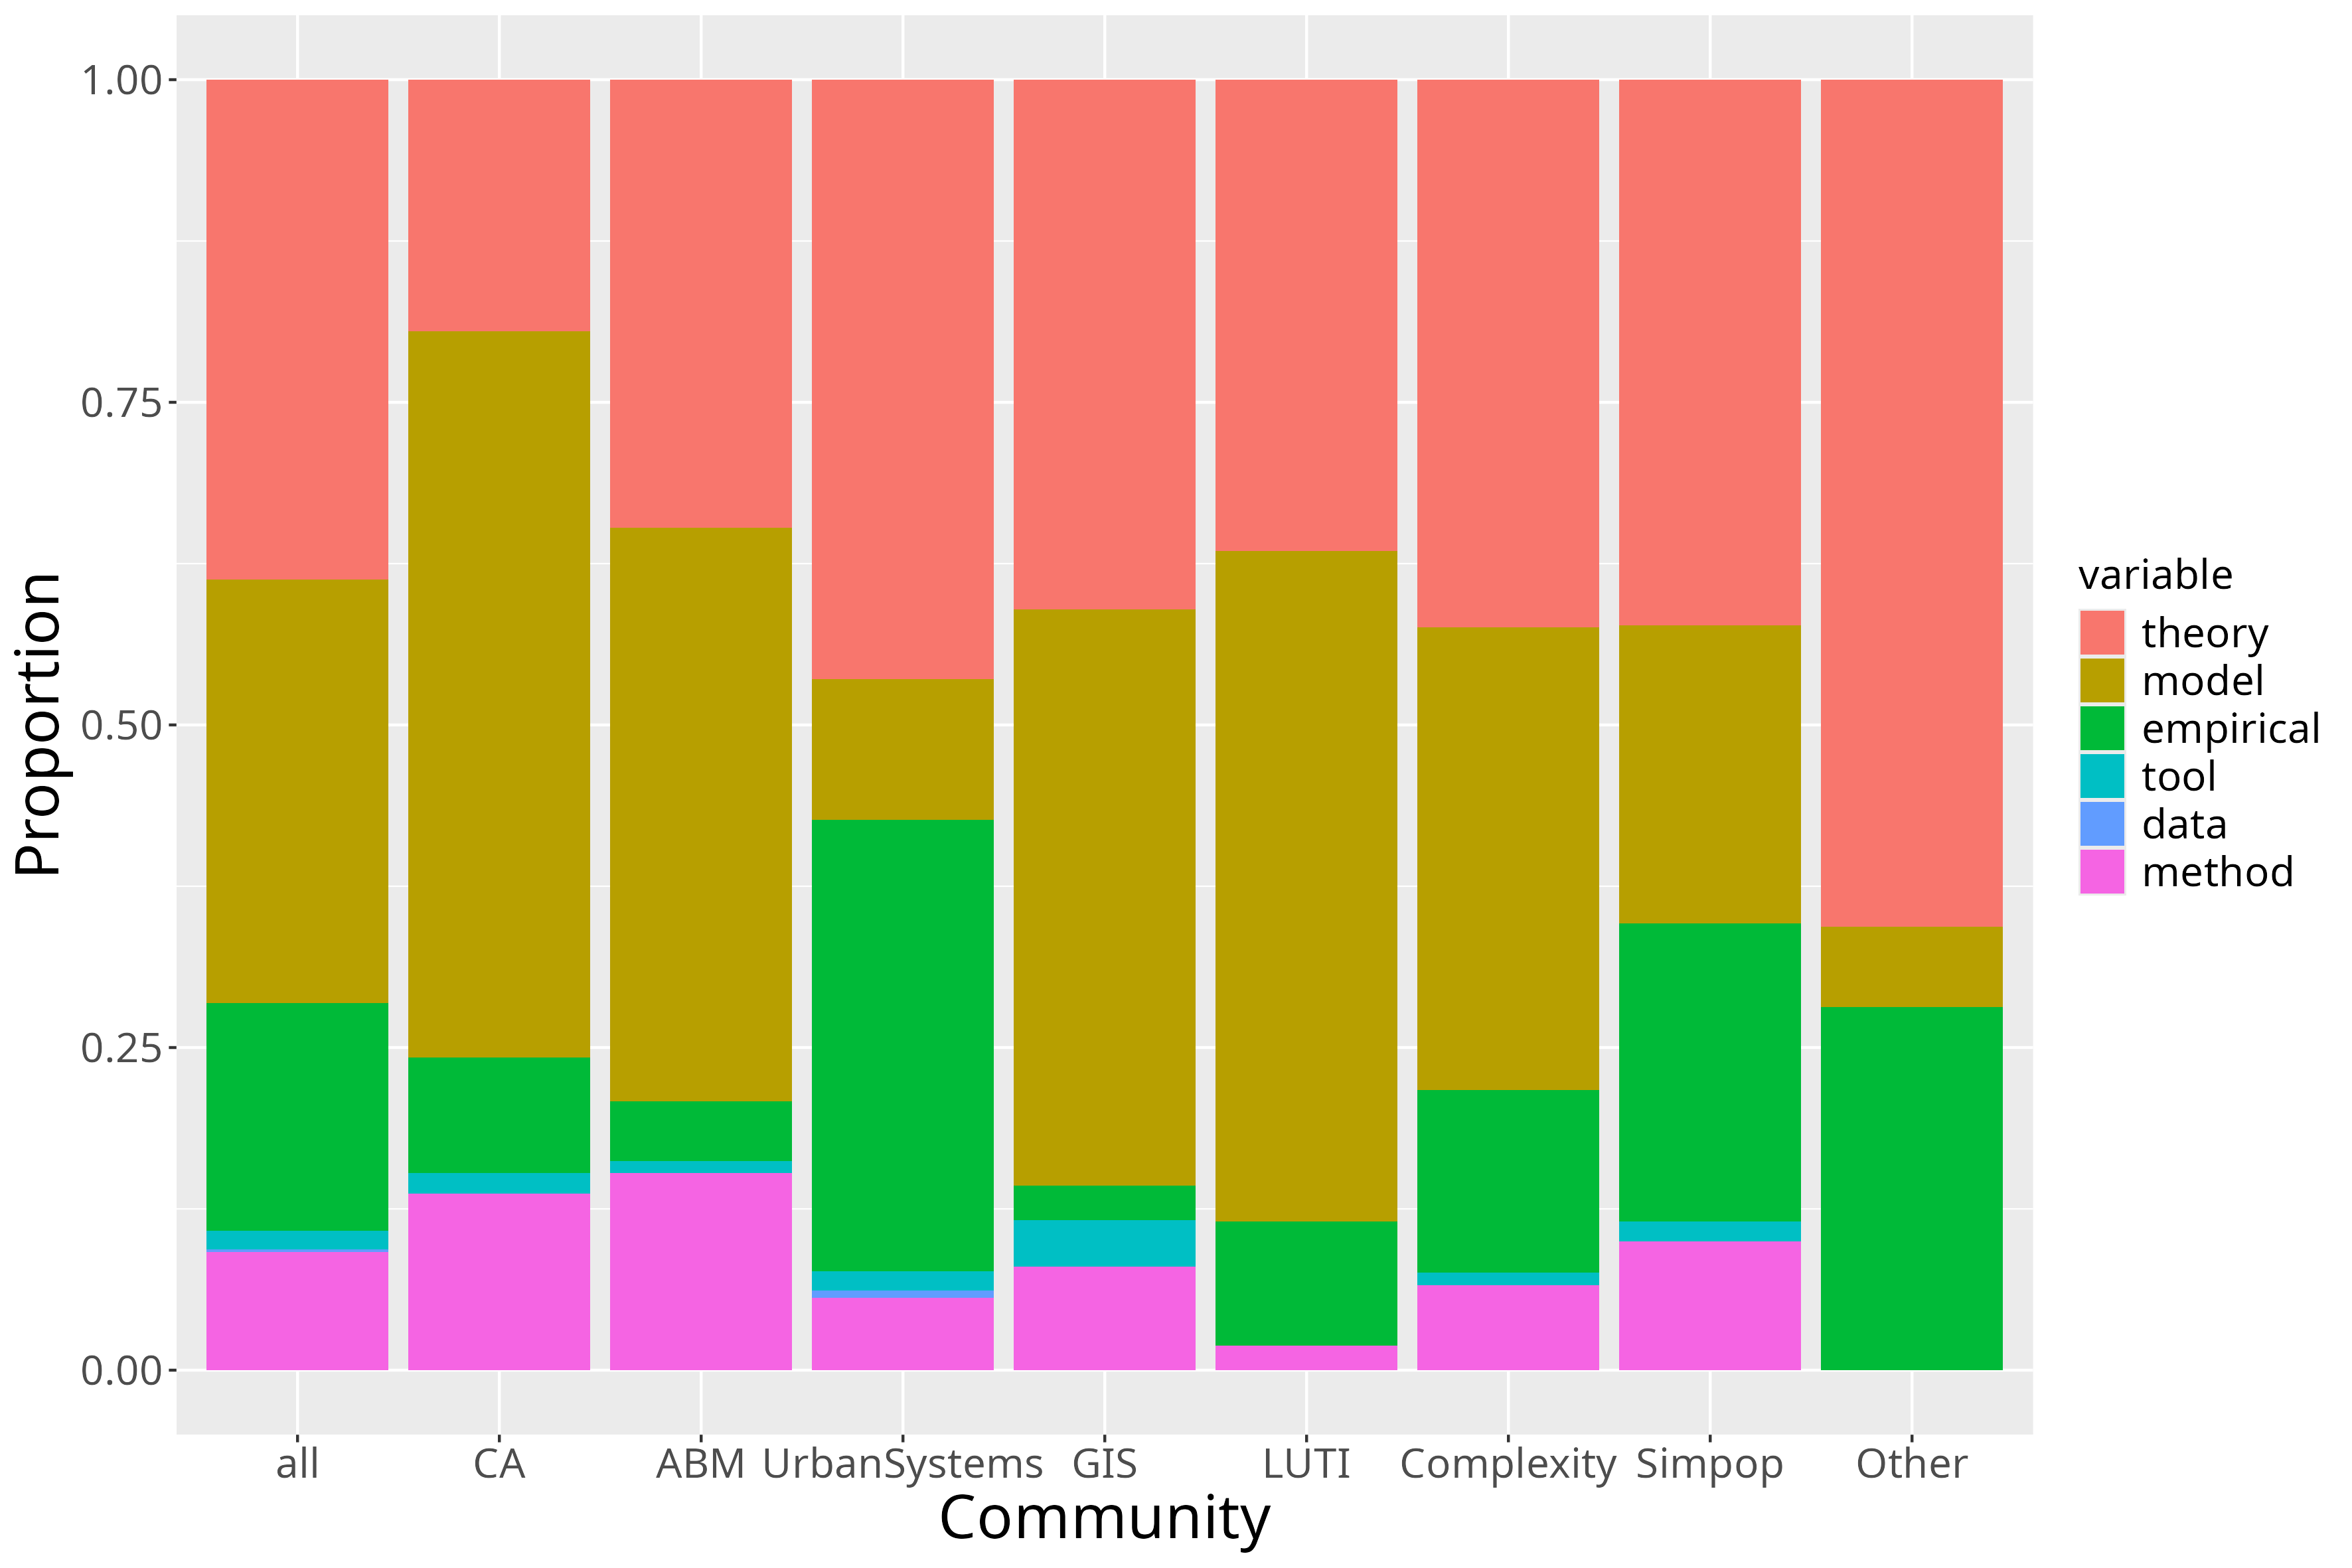
\includegraphics[width=\linewidth]{../../../../Results/evurbth_proportions.png}
\end{center}

\footnotesize

\textit{Composition of communities by Knowledge Domains for the Evolutionary Urban Theory}

}


\sframe{Results: KDs composition}{

\begin{center}
%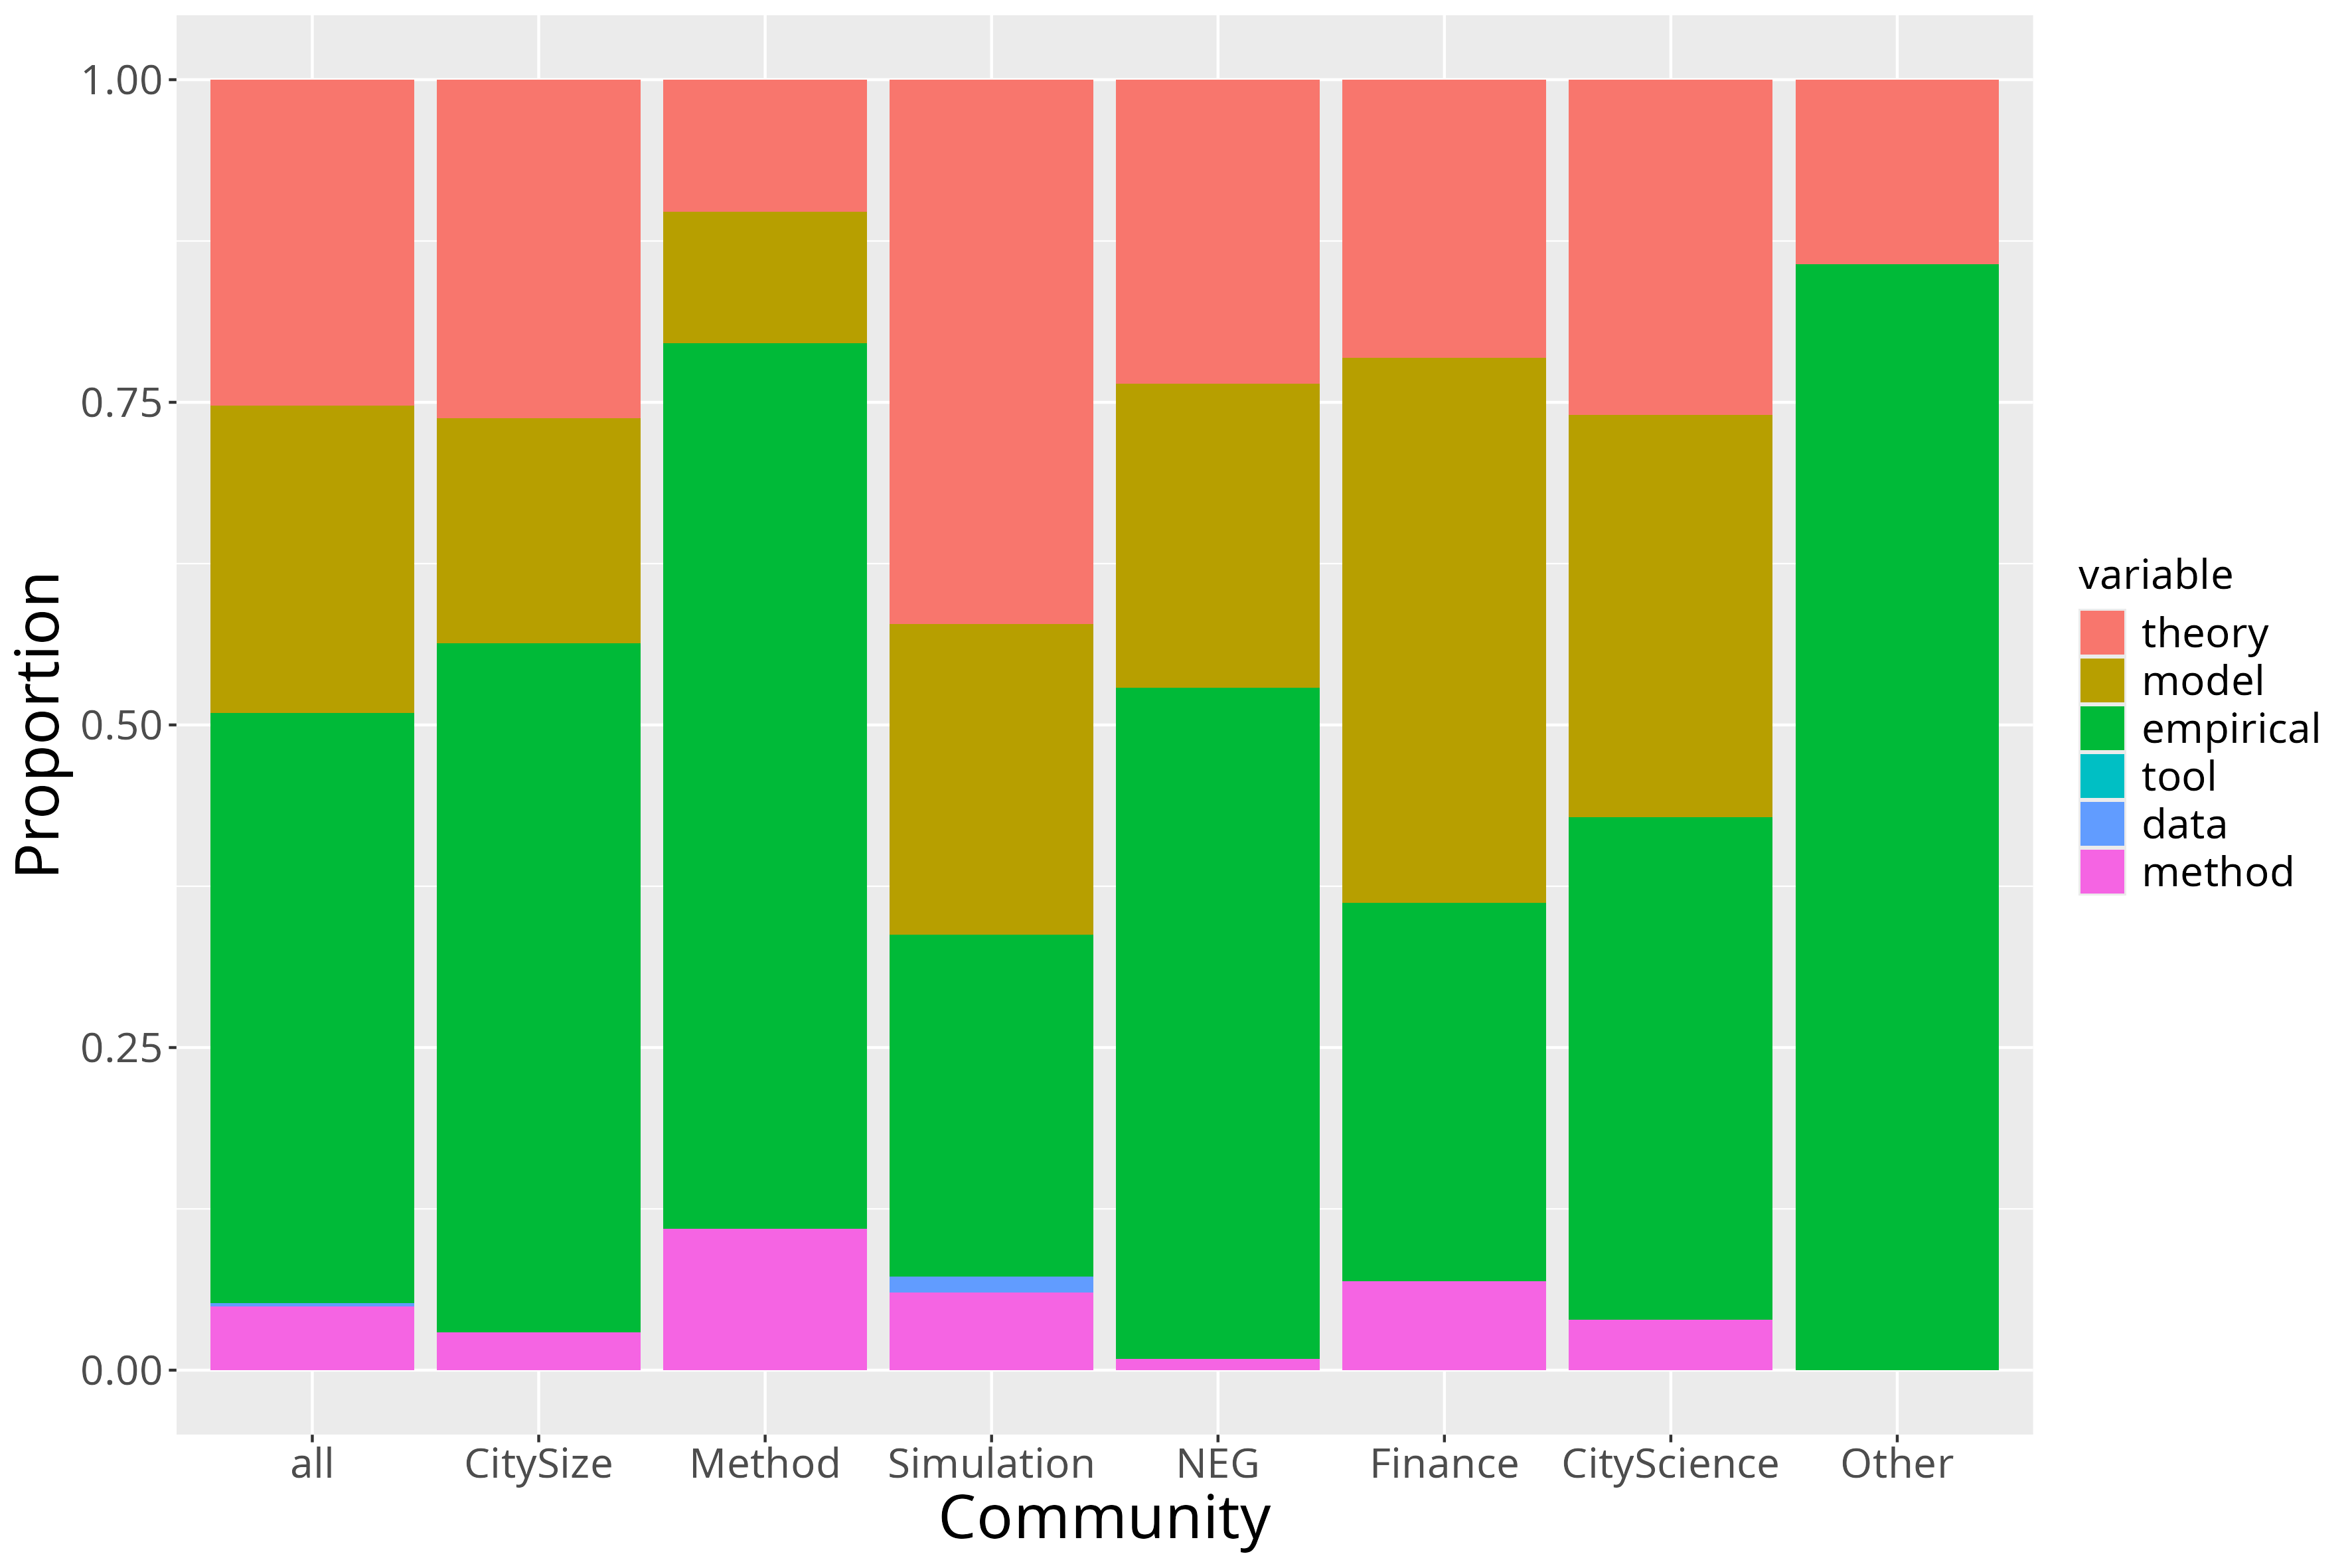
\includegraphics[width=\linewidth]{../../../../Results/zipf_proportions.png}
\end{center}

\footnotesize

\textit{Composition of communities by Knowledge Domains for the Zipf corpus}

}


\sframe{Results: modularities}{

% With the annotated data, we can map interactions between knowledge domains within citations networks, and compute various indicators such as diversity of domains, or modularity in the network capturing how domains are integrated. We find less diversity for Zipf and a much stronger clustering into disciplines with their own use of knowledge domains (theoretical models only in economics for example), while the evolutionary theory witnesses an interdependancy between domains.


% Evolth
%   - communities 0.496  
%   - domains 0.0723
%   - null model -0.0008 +- 0.0049

}



\sframe{Results: key papers}{

% Digging further into this case, we highlight specific papers focused solely on constructing a dataset or presenting a software, on which almost all of the final knowledge depends, confirming this high integration between knowledge domains.


% zoom into the EvolTh citation network

\begin{center}
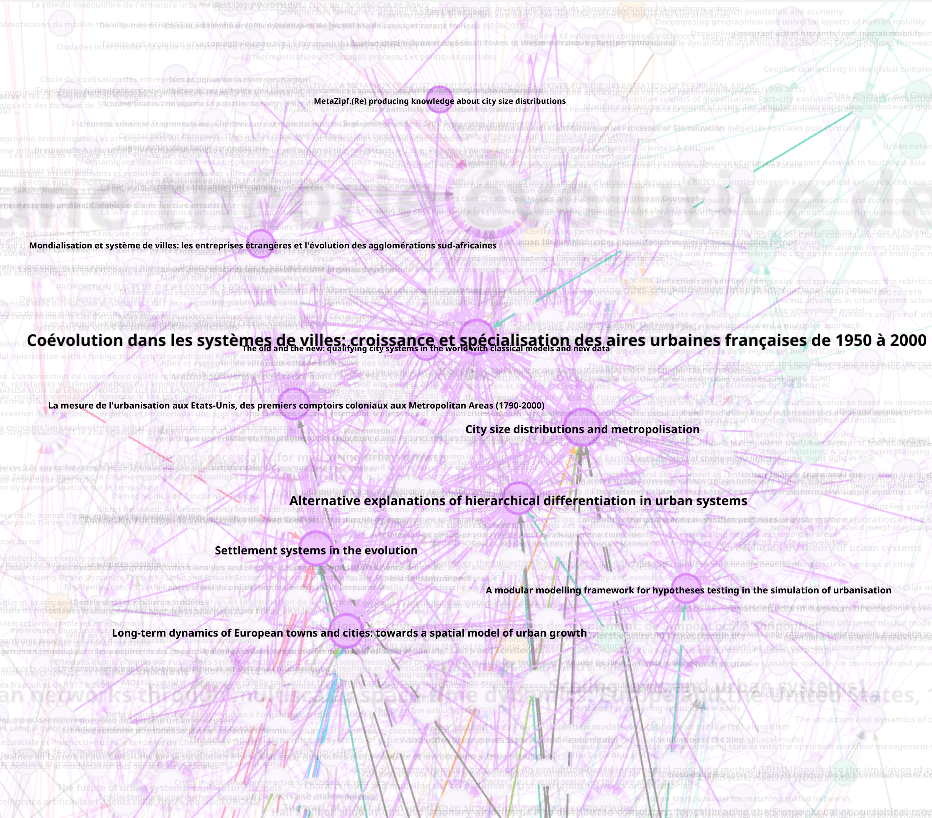
\includegraphics[width=0.45\linewidth]{../../../../Results/zoom_evurbth_geodivercitydata.png}
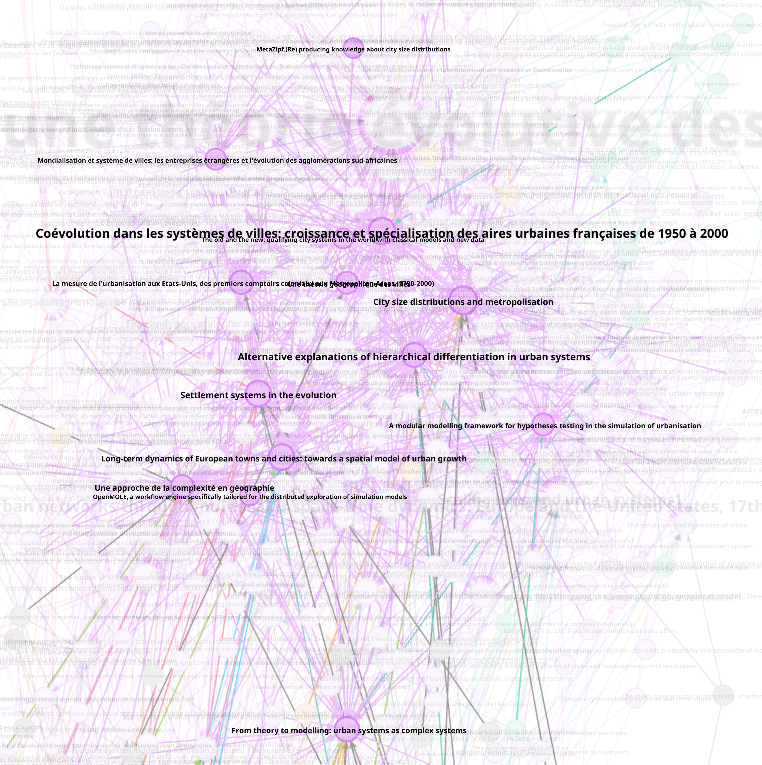
\includegraphics[width=0.45\linewidth]{../../../../Results/zoom_evurbth_openmole.png}
\end{center}


}




\sframe{Perspectives}{


% This contribution thus proposes a first approach in quantitative epistemology to investigate how different components of knowledge interact for the construction of integrated theories. We hypothesise that this aspect is typical in TQG, as our archetypal case study for TQG has shown compared to the more generic case study. Further work would be needed for a broader confirmation of this, with a more systematic mapping of disciplines, without an arbitrary focus on case studies. Sensitivity analysis to the initial definition of corpuses and to the construction of ctation network would also be needed in our case. Finally, an interesting development would be the development of Machine Learning methods to automatically tag papers into knowledge domains, with however a high requirement on classification quality.


% - autres mesures : centralité des differents domaines? (pour influence?)

%\footnotesize

\textbf{Contributions: }
\begin{itemize}
	\item 
\end{itemize}

% not needed as preliminary study?
%\textbf{Work in progress: }
%\begin{itemize}
%	\item 
%\end{itemize}


\textbf{Perspectives: }

\begin{itemize}
	\item 
\end{itemize}


}







%%%%%%%%%%%%%%%%%%%%%
\begin{frame}[allowframebreaks]
\frametitle{References}
\bibliographystyle{apalike}
\bibliography{biblio}
\end{frame}
%%%%%%%%%%%%%%%%%%%%%%%%%%%%



%\begin{frame}{Reserve slides}
%\vfill
%\begin{center}
%{\Huge\bf Reserve slides}
%\end{center}
%\vfill
%\end{frame}




\end{document}

